\chapter{Endelige elementer og endelige element rum}

Når man skal foretage en inddeling af et domæne i planen i endelige
elementer, vælger man af beregningsmæssige hensyn ofte at opdele
området i simple geometriske figurer såsom trekanter eller firkanter. 
Er området ikke-polygonalt kan
man enten vælge at benytte kurvede elementer (se fx
\cite{ciarlet78,johnson87}) eller at foretage en
finere inddeling af området lang randen i mindre trekantet/firkanter.
Endeligt kan man også vælge at afbilde domænet bijektivt på et
``pænere'' domæne. Hvilken fremgangsmåde man vælger er ofte en smagssag.
Traditionelt har man arbejdet med inddelinger i trekanter (eller mere
generelt $n$-simplexer), men firkanter er ved at vinde indpas. I dette
kapitel, hvor vi formelt skal definere endelige elementer og endelige
element rum, vil udgangspunktet være trekanter/$n$-simplexer. I et
senere kapitel, hvor vi skal studere en netinddelings algoritme, vil
rektangler blive anvendt i trianguleringen. Definitionen af nogle af
begreberne i dette kapitel varierer fra forfatter til forfatter.
Fremgangsmåden, vi her skal anvende, kaldes for en konformerende
endelig element metode og er inspireret af \cite{ciarlet78}.

\section{Notation}
Vi skal kort redegøre for notationen vedrørende afledede af funktioner
$v:\R^n \rightarrow \R$. Lad $e_i$, $1\leq i\leq n$ være den
sædvanlige kanoniske basis for $\R^n$. De partielle afledede af $v$
vil da blive betegnet med
\begin{align}
  \p_i v(a) &= Dv(a)e_i, \\
  \p_{ij} v(a) &= D^2 v(a)(e_i,e_j), \\
  \p_{ijk} v(a) &= D^3 v(a)(e_i,e_j,e_k), \\
  \text{osv.} \notag  
\end{align}
Til tider skal vi benytte en multi-indeks notation. Lad
$\alpha=(\alpha_1,\ldots,\alpha_n)\in\NN^n$ og sæt $|\alpha
|=\sum_{i=1}^n \alpha_i$. Ved $\p^{\alpha} v(a)$ vil vi da forstå
resultatet af at anvende den $|\alpha |$'te afledede $D^{|\alpha
|}v(a)$ på en vilkårlig $|\alpha |$-vektor i $(\R^n)^{|\alpha |}$,
hvor basisvektoren $e_i$ forekommer $\alpha_i$ gange $1\leq i\leq n$.
For eksempel for $n=3$ er $\p^{(1,0,0)} v(a)=\p_1 v(a)$,
$\p^{(1,1,1)}v(a)=\p_{123}v(a)$ og $\p^{(3,0,0)}v(a)=\p_{111}v(a)$.
Endelig skal vi også erstatte de kanoniske basisvektorer $e_i$ med
vilkårlige faste vektorer $\xi_i$ for at opnå vilkårlige retningsafledede.
 
\section{Endelige element rum} \label{femindledning}
En væsentlig del af den endelige element metode består af
konstruktionen af endelige dimensionale underrum $\Xfe$ og $\Yfe$ af
løsningsrummet $\X$ hhv. testrummet $\Y$. Fremgangsmåden ved
konstruktionen af $\Xfe$ og $\Yfe$ er selvfølgelig identisk, og vi
skal fremover blot betragte $\Xfe$. Denne konstruktion kan
karakteriseres ved 3 aspekter:
\begin{enumerate}
  \item En triangulering $\Th$ af $\domain$.
  \item For ethvert $K\in \Th$ skal rummet $P_K=\{v|_K \ |\ v\in \Xfe\}$
        indeholde polynomier.
  \item Der skal findes en basis for $\Xfe$, bestående af funktioner
        med så ``lille'' støtte som mulig.
\end{enumerate}
Grunden til at vi forlanger, at rummene $P_K$ skal indeholde polynomier, 
der kan udtrykkes i en basis bestående af funktioner med så ``lille'' støtte
som mulig, er et ønske om dels at få simple beregninger af 
elementerne i (\ref{des1}-\ref{des3}) dels at opnå en matrix, der er
tyndt besat. Vi vil nu studere de tre aspekter i detaljer.

\section{Triangulering af $\overline{\Omega}$} \label{triang}
Man tillader naturligvis ikke vilkårlige inddelinger af domænet. For
at få en sammenhængende teori har følgende definition vist sig at være
fornuftig. 

\begin{definition} \label{defth}
Lad $\overline{\Omega}$ betegne det domæne, hvori en given 
differentialligning søges løst. Ved en triangulering $\Th$ af
$\overline{\Omega}$ forstås en inddeling af $\overline{\Omega}$ i et 
endeligt antal delmængder $K$ på en sådan måde, at følgende betingelser
er opfyldt:
\begin{Thenumerate}
  \item $\overline{\Omega} = \cup_{K\in \Th} K$.
  \item For alle $K\in \Th$ gælder $K = \overline{K}$ og 
        $K^{\circ} \not=\emptyset$. 
  \item For alle $K_1, K_2 \in \Th$ hvor $K_1 \not= K_2$ gælder
        $K_1^\circ \cap K_2^\circ =\emptyset$.
  \item For alle $K \in \Th$ er $\partial K$ Lipschitz kontinuert. 
\end{Thenumerate}
\end{definition}
Vi skal senere tilføje en femte betingelse, der skal være med til at
sikre kontinuitet over randene for naboelementer.
\begin{remark}
Ordet ``endelig'' i den endelige element metode går på opdeling\-en af
$\overline{\Omega}$ i et {\em endeligt} antal delmængder.
\end{remark}
\subsection{Lokale endelige element rum}
For et givet endelig element rum $\Xfe$ (vi skal senere vende tilbage til en
præcis definition) defineres det endelige dimensionale rum $P_K$ som
\begin{equation}
  P_K=\{v|_K \ | \ v\in \Xfe \}.
\end{equation} Som nævnt i kapitel~\ref{variation} vil $\X$ ofte være
$\Het$, $\Hto$ eller lignende. Vi skal nu vise en sætning, der giver 
betingelser, som vil sikre at $\Xfe \subset \Het$.
\begin{theorem} \label{xfehet}
Lad $\dom$ være en åben og begrænset delmængde af $\R^n$. Antag at
inklusionen $P_K \subset \H^1(K)$ holder for alle $K\in \Th$, og at
$\Xfe \subset {\cal{C}}^0(\overline{\Omega})$. Da vil
\begin{gather} 
  \Xfe \subset \H^1(\Omega), \\ 
  {\mathcal X}_{0,{\mathsf{fe}}} = \{ v \in \Xfe \ | \ v = 0 \ \text{på $\p\dom$} \} 
  \subset \H^1_0(\Omega). 
\end{gather}
\end{theorem}
\begin{proof}
Lad $v\in \Xfe$ være givet. Da $\overline{\Omega}$ er begrænset, og da 
$v\in {\cal{C}}^0(\overline{\Omega})$, vil $v\in \Lto$. Ifølge 
definitionen af $\H^1(\Omega)$ vil $v\in \H^1(\Omega)$, såfremt vi for
$i=1,\ldots,n$ kan finde en funktion $v_i \in \Lto$, så der for alle 
$\phi \in {\cal{D}}^{\infty}_{c}(\Omega)$
(${\cal{D}}^{\infty}_{c}(\Omega)$ er mængden af $\infty$-gange
differentiable funktioner med kompakt støtte i $\dom$) gælder 
\begin{equation}
  \int_{\Omega} v_i \phi\, dx = - \int_{\Omega} v\partial_i \phi\, dx .
\end{equation}
Sæt nu $v_i = \partial_i(v|_K)$ for ethvert $K\in \Th$, dvs. $v_i$ er 
restriktionen til ethvert endeligt element $K$ af $\partial_i v$. Da 
ethvert endeligt element $K$ har en Lipschitz kontinuert rand $\partial K$,
kan vi anvende Green's sætning til at få
\begin{equation} 
  \int_K \partial_i(v|_K)\phi\, dx = 
  -\int_K v|_K \partial_i \phi\, dx +
  \int_{\partial K} v|_K \phi \nu_{i,K}\, d\gamma \ \ \text{for alle $K\in \Th$,} 
\end{equation}
hvor $\nu_{i,K}$ betegner den $i$'te komponent i enheds normal vektoren
til $\partial K$. Ved nu at summere over alle endelig elementer fås
\begin{equation}
   \int_{\Omega} v_i \phi\, dx = 
   -\int_{\Omega} v \partial_i \phi\, dx +
   \sum_{K\in \Th} \int_{\partial K} v|_K \phi \nu_{i,K}\, d\gamma 
\end{equation}
Vi bemærker nu, at sidste led på højre siden i ovenstående relation er 0, 
thi enten vil en del af $\partial K$ være en del af $\Omega$'s rand 
$\Gamma$, og så vil $\phi=0$, eller også vil bidraget fra to nabo elementer 
være nul, pga. modsat omløbsretning. Altså haves den første inklusion.
Da randen $\Gamma$ er Lipschitz kontinuert, følger den anden inklusion af
\begin{equation} 
   {\mathcal X}_{0,{\mathsf{fe}}} =\{ v \in \Xfe \ |\ v = 0 
   \ \text{på $\gamma$} \} \subset
   \{ v \in \Het \ |\ v = 0 \ \text{på $\Gamma$} \} = \H^1_0(\Omega). 
\end{equation}
\end{proof}

Beviset for følgende sætning minder meget om beviset for forrige sætning. 
Vi vil derfor nøjes med at angive sætningen.
\begin{theorem} \label{xfeh2}
Lad $\dom$ være en åben og begrænset delmængde af $\R^n$. Antag at
inklusionen $P_K \subset \H^2(K)$ holder for alle $K\in \Th$, og at
$\Xfe \subset {\cal{C}}^1(\overline{\Omega})$. Da vil
\begin{gather}
   \Xfe \subset H^2(\Omega), \\
   {\mathcal X}_{0,{\mathsf{fe}}} = \{ v \in \Xfe\ |\ v = 0 \
   \text{på $\p\dom$} \} 
   \subset \H^2(\Omega) \cap \H^1_0(\Omega), \\
   {\mathcal X}_{00,{\mathsf{fe}}}  = \{ v \in \Xfe \ |\ v = 
   \partial_{\nu}v = 0 \ \text{på $\p\dom$} \} 
   \subset \H^2_0(\Omega), 
\end{gather}
\end{theorem}

\section{Polynomiumsrummene $P_k$}
Vi skal nu definere det polynomiumsrum, der skal bruges i
definitionen af en klasse af endelige elementer.
\begin{definition}
For ethvert $k\geq0$ defineres $P_k^n$ som rummet af polynomier med
$\grad \leq k$ i de $n$ variable $x_1,\ldots,x_n$, dvs. polynomierne $p\in P_k^n$
er afbildninger $p:\R^n\rightarrow \R$ givet ved
\begin{equation}
    p(x)=p(x_1,\ldots,x_n)=
   \sum_{\sum_{i=1}^{n} \alpha_i \leq k} 
   \gamma_{\alpha_1 \cdots \alpha_n} x_1^{\alpha_1}\cdots x_n^{\alpha_n} 
\end{equation}
for passende konstanter $\gamma_{\alpha_1 \cdots \alpha_n}$. 
\end{definition}
\begin{remark}
Vi vil som regel skrive $P_k$ istedet for $P_k^n$, idet dimensionen af
rummet vil fremgå at sammenhængen.
\end{remark}
\begin{remark}
Vi skal til tider benytte os af en mul\-ti-in\-deks no\-ta\-ti\-on og
ud\-tryk\-ke polynomier $p\in P_k$ som
\begin{equation}
   p(x)=\sum_{|\alpha|\leq k} \gamma_{\alpha} x^{\alpha}. 
\end{equation}
\end{remark}
\begin{theorem}
Dimensionen af polynomiumsrummet $P_k^n$ er givet ved 
\begin{equation}
\dim P_k^n = \binom{n+k}{k}. 
\end{equation}
\end{theorem}
\begin{proof}
Det er oplagt, at $x^{\alpha} = x_1^{\alpha_1}\cdots x_n^{\alpha_n}$,
hvor $\alpha_1 + \cdots + \alpha_n \leq k$, $\alpha_i \geq 0$, er en
basis for $P_k^n$. Vi skal så bestemme antallet af måder hvorpå vi kan
vælge $\alpha$'erne så $\alpha_1 + \cdots + \alpha_n = i \leq k$ med
$0 \leq i \leq k$. Dette svarer til valg af $i$ elementer ud af $n$
elementer med tilbagelægning uden hensyn til ordning. Altså er der
\begin{equation}
  \sum_{i=0}^k \binom{n-1+i}{i} = \sum_{i=0}^k \binom{n-1+i}{n-1} = 
  \binom{n+k}{k} 
\end{equation}
muligheder. 
\end{proof}
\begin{definition}
For en delmængde $A\subset \R^n$ sættes
\begin{equation}
P_k(A)=\{p|_A \ |\  p\in P_k\}.
\end{equation}
\end{definition}
\begin{remark}
Hvis $A^\circ \not=\emptyset$, er $\dim P_k = \dim P_k(A)$.
\end{remark}

\section{Lagrange endelige elementer} \label{lagee}
\begin{definition}
Ved et (ikke degenereret) $n$-simplex forstås det konvekse hylster $K$ af 
$n+1$ punkter $a_j=(a_{ij})_{i=1}^n \in \R^n$, også kaldet hjørner,  der
ligger således, at matricen
\begin{equation} 
  {\mathbf A} =
  \left( \begin{array}{cccc}
  a_{11} & a_{12} & \cdots & a_{1,n+1} \\
  a_{21} & a_{22} & \cdots & a_{2,n+1} \\
  \vdots & \vdots &        & \vdots    \\  
  a_{n1} & a_{n2} & \cdots & a_{n,n+1} \\
  1      & 1      & \cdots & 1 
  \end{array} \right)  
\end{equation}
er invertibel.  
\end{definition}
\begin{remark}
Som bekendt er $K$ givet ved
\begin{equation}
   K=\Bigl\{ x=\sum_{j=1}^{n+1} \lambda_j a_j \ \Big| \ 0\leq \lambda_j
   \leq 1, \ 1\leq j \leq n+1, \ \sum_{j=1}^{n+1} \lambda_j =1 \Bigr\}.
\end{equation}
\end{remark}
\begin{remark}
Vi bemærker, at et $2$-simplex er en trekant, og et $3$-simplex er en 
tetraede.
\end{remark}
\begin{definition}
For ethvert tal $m\in\NN_0$ med $0\leq m\leq n$ defineres en $m$-side af et
$n$-simplex $K$ som et $m$-simplex, hvis $m+1$ hjørner også er hjørner i $K$. 
Specielt kaldes en $(n-1)$-side for en side, og en $1$-side kaldes en kant.
\end{definition}
\begin{theorem} \label{p1}
Et polynomium $p \in P_1$ givet ved 
$p : x \rightarrow \sum_{|\alpha|\leq 1} \gamma_{\alpha} x^{\alpha}$ er 
entydig bestemt af dets værdier i de $n-1$ hjørner $a_j$ i et vilkårligt
$n$-simplex $K$ i $\R^n$. 
\end{theorem}
\begin{proof}
Polynomiet $p$ kan skrives på formen $p(x)=\gamma_0 + \gamma_1 x_1 +\cdots+ 
\gamma_n x_n$, hvor vi af notationsmæssige årsager skal kalde $\gamma_0$
for $\gamma_{n+1}$. Lad værdierne $p(a_j)=\mu_j$, $1\leq j\leq n+1$ være
givet. Vi skal da vise, at koefficienterne $\gamma_j$ er entydig bestemt, 
dvs. at ligningssystemet
\begin{equation}
   \mu_j = \gamma_1 a_{1j} + \cdots + \gamma_n a_{nj} + \gamma_{n+1},\ \
   1 \leq j \leq n+1 
\end{equation}
har en entydig løsning. Sættes $\mu=(\mu_1,\ldots,\mu_{n+1})^t$ og 
$\gamma=(\gamma_1,\ldots,\gamma_{n+1})^t$ kan vi skrive ligningssystemet
som
\begin{equation} 
 \mu = {\mathbf A}^t \gamma . 
\end{equation}
Dette system har imidlertid en entydig løsning, da $K$ er et $n$-simplex.
\end{proof}

\begin{remark}
Som en konsekvens af forrige sætning ses, at hvis vi sætter 
$\lambda_i(a_j) = \delta_{ij}$, kan ethvert polynomium 
$p\in P_1$ repræsenteres som 
\begin{equation} 
  p=\sum_{i=1}^{n+1}p(a_i)\lambda_i . 
\end{equation} 
\end{remark}
Vi kan nu definere den simpleste form for et endelig element, 
som vi skal kalde et $n$-simplex af type (1) som værende et 
tripel $\familyfe$ bestående af $n$-simplexet $K$ med hjørner  
$a_j$, rummet $P_K = P_1(K)$, samt mængden $\Sigma_K$ af 
frihedsgrader som består af de parametre, der entydigt definerer 
en funktion i rummet $P_K$, dvs. 
$\Sigma_K = \{ p(a_j)\ |\ 1 \leq j \leq n+1 \}$.

Betegnes midtpunkterne af kanterne i et $n$-simplex med 
$a_{ij}=(a_i+a_j)/2$, kan man efter samme ide som i beviset for sætning
\ref{p1} vise, at polynomier i $P_K=P_2(K)$ har repræsentationen
\begin{equation}
   p=\sum_{i=1}^{n+1}p(a_i)\lambda_i (2\lambda_i-1) + 
     \sum_{\substack{i,j=1 \\ i<j}}^{n+1} p(a_{ij}) 4\lambda_i
     \lambda_j ,  
\end{equation}
hvor $\lambda_k(a_{ij})=(\delta_{ki}+\delta_{kj})/2$, 
$1 \leq i<j \leq n+1$, $1 \leq k \leq n+1$. Heraf fås definitionen
for endnu et endeligt element, kaldet et $n$-simplex af type (2), 
bestående af $K$ som før, rummet $P_K=P_2(K)$ samt $\Sigma_K=\{p(a_i)\ |\ 1\leq
i\leq n+1 \} \cup \{ p(a_{ij})\ |\ 1\leq i<j \leq n+1\}$.

\setlength{\unitlength}{1mm}
\begin{figure}[p]
\begin{center}
\begin{picture}(100,50)(0,0)
\put(5,5){\begin{picture}(40,40)(0,0)
\put(5,5){\line(3,1){30}} \put(5,5){\circle*{1}}
\put(35,15){\line(-1,1){20}} \put(35,15){\circle*{1}}
\put(5,5){\line(1,3){10}} \put(15,35){\circle*{1}}
\end{picture}}
\put(55,5){\begin{picture}(40,40)(0,0)
\put(5,15){\line(1,2){10}} \put(5,15){\circle*{1}}
\put(5,15){\line(2,-1){20}} 
\put(25,5){\line(1,2){10}} \put(25,5){\circle*{1}}
\put(35,25){\line(-2,1){20}} \put(35,25){\circle*{1}}
\put(15,35){\line(1,-3){10}} \put(15,35){\circle*{1}}
\dashline{2}(5,15)(35,25)
\end{picture}}
\end{picture}
\end{center}
\caption{Trekant af type $(1)$ og tetraede af type $(1)$\label{fe1}}
\end{figure}
\setlength{\unitlength}{1mm}
\begin{figure}[p]
\begin{center}
\begin{picture}(100,50)(0,0)
\put(5,5){\begin{picture}(40,40)(0,0)
\put(5,5){\line(1,0){20}} \put(5,5){\circle*{1}}
\put(5,5){\line(1,1){30}} \put(25,5){\circle*{1}}
\put(25,5){\line(1,3){10}} \put(35,35){\circle*{1}}
\dashline{2}(15,5)(20,20) \put(15,5){\circle*{1}}
\dashline{2}(15,5)(30,20) \put(20,20){\circle*{1}}
\dashline{2}(20,20)(30,20) \put(30,20){\circle*{1}}
\end{picture}}
\put(55,5){\begin{picture}(40,40)(0,0)
\put(5,5){\line(1,0){20}} \put(5,5){\circle*{1}}
\put(5,5){\line(1,3){10}} \put(25,5){\circle*{1}}
\put(25,5){\line(-1,3){10}} \put(15,35){\circle*{1}}
\put(25,5){\line(1,2){10}} \put(35,25){\circle*{1}}
\put(15,35){\line(2,-1){20}}
\put(15,5){\circle*{1}} % 
\dashline{2}(10,20)(15,5)
\put(10,20){\circle*{1}} % 
\dashline{2}(10,20)(20,20)
\put(20,20){\circle*{1}} % 
\dashline{2}(20,20)(15,5)
\put(20,15){\circle*{1}} % 
\dashline{2}(20,15)(30,15)
\put(30,15){\circle*{1}} % 
\dashline{2}(20,15)(25,30)
\put(25,30){\circle*{1}} % 
\dashline{2}(25,30)(30,15)
\dashline{2}(5,5)(35,25)
\end{picture}}
\end{picture}
\end{center}
\caption{Trekant af type $(2)$ og tetraede af type $(2)$\label{fe2}}
\end{figure}
\setlength{\unitlength}{1mm}
\begin{figure}[p] 
\begin{center}
\begin{picture}(130,55)(0,0)
\put(0,0){\begin{picture}(55,40)(0,0)
\put(20,5){\line(1,0){30}} \put(20,5){\circle*{1}}
\put(20,5){\line(-1,2){15}} \put(5,35){\circle*{1}}
\put(50,5){\line(-3,2){45}} \put(50,5){\circle*{1}}
\put(30,5){\circle*{1}}
\put(40,5){\circle*{1}}
\put(15,15){\circle*{1}}
\put(25,15){\circle*{1}}
\put(35,15){\circle*{1}}
\put(10,25){\circle*{1}}
\put(20,25){\circle*{1}}
\dashline{2}(15,15)(35,15)
\dashline{2}(10,25)(20,25)
\dashline{2}(15,15)(30,5)
\dashline{2}(10,25)(40,5)
\dashline{2}(20,25)(30,5)
\dashline{2}(35,15)(40,5)
\end{picture}}
\put(60,0){\begin{picture}(70,55)(0,0)
\put(5,5){\line(1,0){30}}
\put(5,5){\line(1,2){15}}
\put(35,5){\line(-1,2){15}}
\put(35,5){\line(2,3){30}}
\put(20,35){\line(3,1){45}}
\put(5,5){\circle*{1}} \put(15,5){\circle*{1}}
\put(25,5){\circle*{1}} \put(35,5){\circle*{1}}
\put(10,15){\circle*{1}} \put(20,15){\circle*{1}}
\put(30,15){\circle*{1}} \put(15,25){\circle*{1}}
\put(25,25){\circle*{1}} \put(20,35){\circle*{1}}
\put(25,20){\circle*{1}} \put(35,20){\circle*{1}}
\put(45,20){\circle*{1}} \put(30,30){\circle*{1}}
\put(40,30){\circle*{1}} \put(35,40){\circle*{1}}
\put(45,35){\circle*{1}} \put(55,35){\circle*{1}}
\put(50,45){\circle*{1}} \put(65,50){\circle*{1}}
\dashline{2}(10,15)(30,15) \dashline{2}(15,25)(25,25)
\dashline{2}(10,15)(15,15) \dashline{2}(15,25)(25,5)
\dashline{2}(15,5)(25,25) \dashline{2}(25,5)(30,15)
\dashline{2}(25,20)(45,20) \dashline{2}(30,30)(40,30)
\dashline{2}(25,20)(35,40) \dashline{2}(45,20)(35,40)
\dashline{2}(30,30)(35,20) \dashline{2}(40,30)(35,20)
\dashline{2}(45,35)(55,35) \dashline{2}(45,35)(50,45)
\dashline{2}(50,45)(55,35) \dashline{2}(5,5)(65,50)
\end{picture}}
\end{picture}
\end{center}
\caption{Trekant af type $(3)$ og tetraede af type $(3)$\label{fe3}}
\end{figure}

Lad $K$ være et $n$-simplex med hjørner $a_1,\ldots,
a_{n+1}$. Sættes $a_{iij}=(2a_i+a_j)/3$ for $i\not= j$ og 
$a_{ijk}=(a_i+a_j+a_k)/3$ for $i<j<k$ kan man (igen på tilsvarende måde
som i sætning~\ref{p1}) vise, at polynomier i $P_3(K)$ har formen
\begin{multline}
\forall p\in P_3, \ 
p = \sum_i \frac{\lambda_i(3\lambda_i -1)(3\lambda_i -2)}{2}p(a_i) \\
+ \sum_{i\not= j} \frac{9\lambda_i \lambda_j(3\lambda_i -1)}{2}p(a_{iij})
+ \sum_{i<j<k} 27\lambda_i \lambda_j \lambda_k p(a_{ijk}).
\end{multline}
Dette giver os et $n$-simplex af type (3). Figurerne~\ref{fe1},
\ref{fe2} og \ref{fe3} viser eksempler på nogle af de mest anvendte
endelige elementer. 
For at kunne give en generel definition har vi brug for nedenstående
sætning. Beviset for sætningen er ret teknisk og ikke interessant i
sig selv, hvorfor vi vil undlade det.

\begin{theorem} \label{pk}
Lad $K$ være et $n$-simplex med hjørner $a_j$, $1 \leq j \leq n+1$
Da vil et vilkårlig polynomium $p \in P_k$ være entydigt bestemt af 
dets værdier i punkterne givet 
\begin{multline}
  L_k(K) = \Bigl\{ x = \sum_{j=1}^{n+1} \gamma_j a_j \ \Big| \ 
  \sum_{j=1}^{n+1} \gamma_j = 1, \\
  \gamma_j \in  \Bigl\{ 0, \frac{1}{k},\ldots,\frac{k-1}{k},1 \Bigr\}, \
  1 \leq j \leq n+1 \Bigr\}. 
\end{multline}
\end{theorem}
\begin{proof}
Se fx~\cite{nico}. 
\end{proof}

\begin{remark}
Mængden $L_k(K)$ kaldes for hovedgitteret af orden $k$ for 
$n$-simplexet $K$.
\end{remark}
Vi kan nu give en generel definition af en bestemt klasse af endelige
elementer også kaldet $n$-simplexer af type $(k)$.
\begin{definition}
Ved et $n$-simplex af type $(k)$ forstås et tripel $\familyfe$
be\-stå\-en\-de af et $n$-simplex $K$ med hjørner $a_j, \ 1 \leq j \leq n+1$, 
polynomiumsrummet $P_K=P_k(K)$ samt mængden af frihedsgrader
$\Sigma_K = \{ p(x)\ |\ x \in L_k(K) \}$.
\end{definition}
\begin{definition}
Endelige elementer, hvor frihedsgraderne udelukkende er punkt\-værdier,
kaldes for Langrange endelige elementer.
\end{definition}

\subsection{Triangulering af $\overline{\dom}$ med simplexer}
Vi skal nu se nærmere på, hvorledes man konstruerer en 
triangulering af $\Omega$ med de endelig elementer, der er blevet defineret
i afsnit~\ref{lagee}. Som nævnt i afsnit~\ref{triang} vil vi tilføje
et femte krav til de fire fra definition~\ref{defth}.
Da ikke-degenererede $n$-simplexer er afsluttede, har et ikke tomt indre og en 
Lipschitz kontinuert rand, vil betingelserne $\Th 2.$ og $\Th 4.$ 
altid være opfyldte. Vi behøver derfor kun at koncentrere os om at 
opdele $\Omega$, så betingelserne $\Th 1.$ og $\Th 3.$ er opfyldt. Vi skal
nu stille endnu et krav til en triangulering af $\Omega$. Dette krav
skal sikre, at $\Xfe \subset {\cal{C}}^0(\overline{\Omega})$, og senere
hen at $\Xfe \subset {\cal{C}}^1(\overline{\Omega})$.
\begin{definition} \label{th5}
For at sikre en fornuftig definition af endelige element rum har vi brug 
for følgende ekstra krav til trianguleringen af $\domain$
\begin{Thenumerate}
 \setcounter{enumi}{4}
 \item En vilkårlig side i et vilkårlig $n$-simplex $K_1$ i en given
       triangulering er enten en delmængde af randen $\p\dom$ eller en 
       side i et andet $n$-simplex $K_2$.
\end{Thenumerate}
\end{definition}
\begin{remark}
Betingelsen $\Th 5$ er teoretisk ideel, idet den er med til at sikre
kontinuitet i den endelige element løsning over randene mellem de
enkelte elementer. I praktiske
situationer er den ikke nødvendig, for at den endelige element metode
fungerer. Måske er man end ikke interesseret i en løsning, der er
kontinuert over randene. 
Man kan også få kontinuitet over kanterne uden denne
betingelse, hvis blot man er mere påpasselig med at vælge
polynomiumsrummene $P_K$ i de enkelte elementer $K$. I
figurerne~\ref{lov} og \ref{ulov} ses eksempler
på en tilladt triangulering og en ikke-tilladt triangulering.
\end{remark}
\begin{figure}[htb]
\noindent
\begin{minipage}[b]{.45\linewidth}
  \centering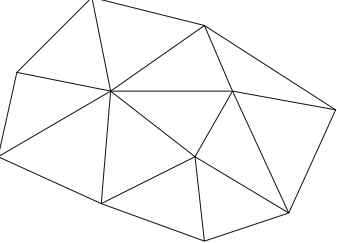
\includegraphics[width=\linewidth]{lovnet}
  \caption{Eksempel på tilladt triangulering\label{lov}} 
\end{minipage}\hfill
\begin{minipage}[b]{.45\linewidth}
  \centering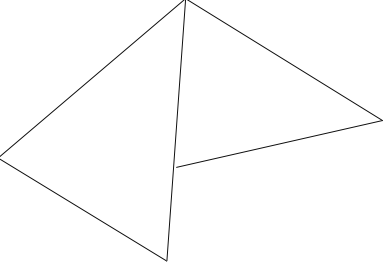
\includegraphics[width=\linewidth]{ulovnet}
  \caption{Eksempel på ikke-tilladt triangulering\label{ulov}} 
\end{minipage}
\end{figure}
\begin{remark}
Har to $n$-simplexer $K_1$ og $K_2$ en fælles side, kaldes $K_1$ og
$K_2$ naboelementer (eng. adjacent).
\end{remark}

\section{Endelige element rum hørende til $n$-sim\-plex\-er af type $(k)$}
Vi er nu i stand til at give en definition af endelige element rum
hørende til $n$-simplexer af type $(k)$.
\begin{definition}
Lad $\Th$ være en triangulering af $\overline{\Omega}$. Ved et endeligt
element rum $\Xfe$ hørende til $n$-simplexer af type $(k)$ forstås en
mængde af funktioner $v: \overline{\Omega} \rightarrow \R$ opfyldende 
følgende krav
\begin{enumerate}
 \item restriktionen af $v$ til $K$ tilhører $P_k(K)$ for alle
       $K\in \Th$.
 \item funktionen $v$ er entydigt bestemt ved dens værdier i punkterne
       \begin{equation}
         \Sigma_h = \{ v(x)\ |\ x \in \cup_{K\in \Th} L_k(K) \}.
       \end{equation}
\end{enumerate}
Mængden $\Sigma_h$ kaldes mængden af frihedsgrader for det endelige 
element rum $\Xfe$.
\end{definition}
\begin{remark}
På grund af betingelse $\Th 5$.\ er der ingen flertydighed i definitionen
af frihedsgraderne.
\end{remark}
\begin{theorem}
Lad $\Xfe$ være det endelige element rum hørende til $n$-sim\-plex\-er
af type $(k)$. Da vil
\begin{equation} 
\Xfe \subset {\cal{C}}^0(\overline{\Omega}) \cap \Het .
\end{equation}
\end{theorem}
\begin{proof}
Lad $K_1$ og $K_2$ være to $n$-simplexer af type $(k)$ med fælles side
$K'$, hvor $K_1$ er bestemt af punkterne $a_1,\ldots,a_{n+1}$ og $K_2$ 
af punkterne $b_1,\ldots,b_{n+1}$. Da $K_1$ og $K_2$ har en fælles 
side $K'$ vil $n$ af punkterne $a_1,\ldots,a_{n+1}$ være identiske med
$n$ af punkterne $b_1,\ldots,b_{n+1}$. Disse $n$ sammenfaldende 
punkter er præcis de punkter, der udspænder $(n-1)$-simplexet $K'$.
Vi bemærker, at $L_k(K')\subset L_k(K_1)$ og $L_k(K')\subset L_k(K_2)$.
For en given funktion $v\in \Xfe$ betragtes nu funktionerne $v|_{K_1}$ 
og $v|_{K_2}$ på den fælles side $K'$. Vi indfører koordinatsystemet
$t=(t_1,\ldots,t_{n-1})$ på $K'$ betragtet som hyperplan. Betragtet som
funktion af $t$ er $v|_{K_1}$ og $v|_{K_2}$ $k$'te grads polynomier
på $K'$, der stemmer overens i de $\binom{n+k}{k}$ 
punkter i $L_k(K')$. Altså må $v|_{K_1}$ og $v|_{K_2}$ være identiske
på $K'$ ifølge sætning~\ref{pk}, og dermed $\Xfe \subset {\cal
C}^0(\domain)$. Inklusionen $\Xfe\subset\H^1(\Omega)$ følger af
sætning~\ref{xfehet}. Figur~\ref{special} illustrerer tilfældet, hvor $n=2$ og
trekanter af type $(2)$ 
\end{proof}

\setlength{\unitlength}{1mm}
\begin{figure}[htb]
\begin{center}
\begin{picture}(55,60)(0,0)
\put(25,30){\line(1,-3){8}}
\put(25,30){\line(-1,3){8}}
\put(5,20){\line(5,-1){25}}
\put(5,20){\line(3,5){15}}
\put(30,15){\line(2,1){20}}
\put(20,45){\line(3,-2){30}}
\put(5,20){\circle*{1}}
\put(30,15){\circle*{1}}
\put(40,20){\circle*{1}}
\put(50,25){\circle*{1}}
\put(35,35){\circle*{1}}
\put(20,45){\circle*{1}}
\put(25,30){\circle*{1}}
\put(17.5,17.5){\circle*{1}}
\put(12.5,32.5){\circle*{1}}
\thicklines
\put(25,30){\line(1,-3){5}}
\put(25,30){\line(-1,3){5}}
\put(20.5,45.5){\makebox(0,0)[bl]{$a_i$}}
\put(25.5,30.5){\makebox(0,0)[bl]{$a_{ij}$}}
\put(31.5,13){\makebox(0,0)[bl]{$a_j$}}
\put(15,25){\makebox(0,0){$K_1$}}
\put(40,25){\makebox(0,0){$K_2$}}
\put(20,35){\makebox(0,0){$K^{'}$}}
\put(33,5){\makebox(0,0)[l]{$(t)$}}
\end{picture}
\end{center}
\caption{Illustation for situationen $n=2$ og trekant af type $(2)$\label{special}}
\end{figure}

\section{Basisfunktioner for endelige element rum}
I afsnit~\ref{femindledning} pointerede vi vigtigheden af, at
basisfunktionerne for
endelige element rum havde så ``lille'' støtte som muligt. For
endelige element rum hørende til $n$-simplexer af type $(k)$ er
mængden af frihedsgrader $\Sigma_h$ givet ved
\begin{equation}
  \Sigma_h = \{ v(x_j) \ |\ 1\leq j\leq M \},
\end{equation}
hvor punkterne $x_j, \ j=1,\ldots,m$ er punkterne i $\cup_{K\in\Th} L_k(K)$.
Det er oplagt, at funktionerne $\phi_i$, $1\leq i\leq M$ defineret ved
betingelserne 
\begin{equation}
  \phi_i \in\Xfe \quad \text{og} \quad \phi_i(x_j)=\delta_{ij}, \
  1\leq i,j\leq M,
\end{equation}
udgør en basis for $\Xfe$, og at støtten for disse funktioner er
``lille''. Figur~\ref{support} indeholder et eksempel på støtten for
basisfunktioner hørende til $n$-simplexer af type $(2)$.
\begin{figure}[htbp]
  \setlength{\unitlength}{1bp}
  \begin{center}
    \begin{picture}(241,256)(0,0)
      \put(1,1){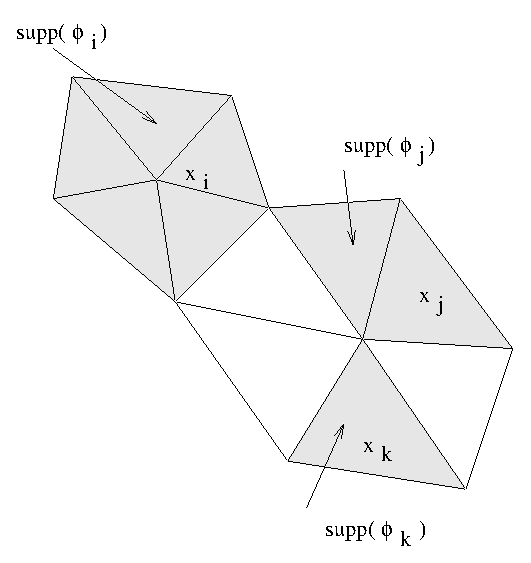
\includegraphics{support}}
    \end{picture}
  \end{center}
  \caption{Eksempel på støtte for basisfunktioner hørende til
$n$-simplexer af type $(2)$\label{support}}   
\end{figure}

\section{Hermite endelige elementer}
Vi skal nu se et eksempel på et endelig element, hvor frihedsgraderne
ikke udelukkende er punktværdier, men også retningsafledede.

\begin{theorem} \label{sec:arg} \label{argee}
Lad $K$ være en trekant med hjørner $a_i, \ i=1,2,3$, hvor sidernes 
midtpunkter betegnes med $a_{ij}=(a_i+a_j)/2, \ 1\leq i<j\leq 3$.
Da vil ethvert polynomium af grad 5 være entydig bestemt ved dets 
værdier i mængden af de 21 frihedsgrader 
\begin{equation} 
\Sigma_K = \Bigl\{ \partial^{\alpha}p(a_i), \ |\alpha| \leq 2, \ 1\leq i\leq 3; \ 
\afl{p(a_{ij})}{\n} ,\ 1\leq i<j\leq 3 \Bigr\}, 
\end{equation}
hvor $\afl{}{\n}$ betegner den normal afledede langs randen af $K$. 
\end{theorem}
\begin{proof}
Lad $p\in P_5(K)$
Da dimensionen af $P_5(K)$ er lig med antallet af frihedsgrader $(=21)$, er 
det nok at vise, at hvis værdien i alle frihedsgraderne er 0, da vil
$p\equiv 0$. Hvis $s$ betegner retningen af siden $a_2a_3$ vil
\begin{equation} \label{sec:arg1}
  p(a_i) = \afl{p}{s}(a_i) = \frac{\partial^2 p}{\partial s^2}(a_i)
  =0, \quad i=2,3. 
\end{equation}
Da $p$ er et polynomium af grad højest 5 på siden $a_2a_3$, må
$p\equiv 0$ på
$a_2a_3$. På $a_2a_3$ er $\afl{p}{\n}$ et polynomium af grad højest 4 og
\begin{equation} \label{sec:arg2}
  \afl{p}{\n}(a_{23})=\afl{p}{\n}(a_i)=
  \frac{\partial}{\partial s}\Bigl(\afl{p}{\n}\Bigr)(a_i)=0, \quad i=2,3 
\end{equation}
hvilket kun er muligt, hvis $\afl{p}{\n}=0$ på $a_2a_3$. Altså er både
$p$ og $\afl{p}{\n}$ identisk 0 på $a_2a_3$, hvilket betyder, at vi kan
faktorisere $(\lambda_1(x))^2$ ud af $p$. Vi har derfor
\begin{equation} 
  p(x)=(\lambda_1(x))^2 p_3(x), 
\end{equation}
hvor $p_3\in P_3(K)$. På tilsvarende vis ses, at vi kan faktorisere 
$(\lambda_2(x))^2$ og $(\lambda_3(x))^2$ ud, hvorfor
\begin{equation} 
  p=\gamma \lambda_1^2 \lambda_2^2 \lambda_3^2 , 
\end{equation}
hvor $\gamma$ er en passende konstant. Da $p\in P_5(K)$ er denne 
faktorisering kun mulig såfremt $\gamma =0$, og dermed er $p\equiv 0$ på $K$. 
\end{proof}

\begin{definition} 
Det endelige element $(K,P_5(K),\Sigma_K)$, hvor $K$ og $\Sigma_K$ er som
i sætning~\ref{argee}, kaldes også Argyris' trekant, se figur~\ref{argtrekant}.
\end{definition}
\begin{figure}[htbp]
  \setlength{\unitlength}{1bp}
  \begin{center}
    \begin{picture}(376,175)(0,0)
      \put(1,1){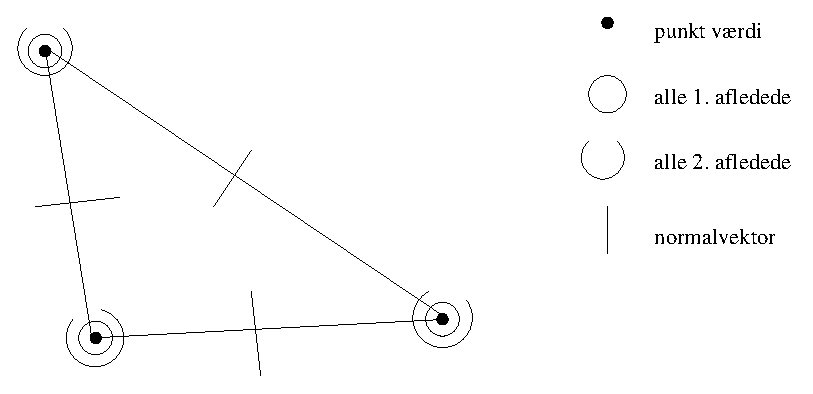
\includegraphics{argyris}}
    \end{picture}
  \end{center}
  \caption{Argyris' trekant\label{argtrekant}}
\end{figure}
\begin{theorem}
Lad $\Xfe$ være det endelig element rum as\-so\-ci\-e\-ret med Ar\-gy\-ris' tre\-kant. 
Da vil
\begin{equation} 
  \Xfe \subset {\cal{C}}^1(\overline{\Omega}) \cap \Hto .
\end{equation}
\end{theorem}
\begin{proof}
Ifølge sætning~\ref{xfeh2} er det nok at vise 
$X_h \subset {\cal{C}}^1(\overline{\Omega})$. Lad $K_1$ og $K_2$ være
to nabo trekanter med fælles side $K'$ og lad $p_i, \ i=1,2$ være 
to funktioner i $\Xfe$ med
\begin{gather}
  \partial^{\alpha}p_1 = \partial^{\alpha}p_2 
  \ \text{i $K'$s endepunkter, $|\alpha|\leq 2$,} \\
  \afl{p_1}{\n} = \afl{p_2}{\n} \ \text{i $K'$s midtpunkt,} 
\end{gather}
hvor $\afl{}{\n}$ betegner differentation i normal retningen til $K'$.
Det følger nu af \eqref{sec:arg1} og \eqref{sec:arg2} fra
sætning~\ref{sec:arg}, at vi for differensen $p=p_1-p_2$ har
\begin{equation} \label{afl1}
 p\equiv \afl{p}{n}\equiv 0 \ \text{på $K'$,} 
\end{equation}
og da $p\equiv 0$ på $K'$ må 
\begin{equation} \label{afl2}
\afl{p}{s}\equiv 0 ,
\end{equation}
hvor $\afl{}{s}$ betegner differentation i retningen tangentielt til
$K'$. Det følger nu af \eqref{afl1} og \eqref{afl2}, at funktionerne $p_i$
samt deres første afledede varierer kontinuert over $K'$, så 
$\Xfe \subset {\cal{C}}^1(\overline{\Omega})$.
\end{proof}
\begin{definition}
Endelige elementer, hvor frihedsgraderne består af punktværdier og
retningsafledede, kaldes Hermite endelige elementer.
\end{definition}

\section{Generelle endelige elementer}
For at kunne give en generel definition af endelige elementer har vi
brug for følgende definition, der kan ses som en generalisering af
begrebet frihedsgrader.
\begin{definition}
Lad $F$ være en mængde af funktioner med reelle værdier defineret på
en mængde $A$, og lad $\Theta$ være en mængde af lineært uafhængige 
lineære afbildninger $\theta_i, \ 1\leq i \leq N$ defineret på $F$. 
$\Theta$ kaldes da $F$-unisolvent, hvis der for givne reelle tal
$\alpha_i, \ 1\leq i \leq N$ findes en entydig funktion $f\in F$, som
opfylder
\begin{equation}
 \theta_i(f) = \alpha_i, \quad 1\leq i \leq N.
\end{equation}
\end{definition}
\begin{definition} \label{genee}
Et endelig element i $\R^n$ er et tripel $(K,P,\Sigma)$, hvor
\begin{enumerate}
  \item $K$ er en afsluttet delmængde af $\R^n$ med et ikke tomt indre
        og en Lipschitz kontinuert rand.
  \item P er en mængde af funktioner med reelle værdier defineret på $K$.
  \item $\Sigma$ er en $P$-unisolvent mæng\-de af li\-ne\-ært
        u\-af\-hæn\-gi\-ge, li\-ne\-ære af\-bild\-ning\-er 
        $\phi_i$, \newline $1\leq i \leq N$ defineret på $P$.
\end{enumerate}
\end{definition}
\begin{remark}
På grund af betingelse (3) i definition~\ref{genee} findes der funktioner $p_i, \
1\leq i \leq N$, som opfylder
\begin{equation}
  \phi_j (p_i) = \delta_{ij}, \quad 1\leq j \leq N,
\end{equation}
så polynomier $p\in P$ kan skrives på formen
\begin{equation}
  p = \sum_{i=1}^N \phi_i(p)p_i .
\end{equation}
Altså er funktionsrummet $P$ endelig dimensionalt, og $\dim P=N$.
\end{remark}
\begin{definition}
De lineære afbildninger $\phi_i, \ 1\leq i\leq N$ kaldes
frihedsgraderne for det endelige element $\fe$, og funktionerne $p_i, \
1\leq i\leq N$ kaldes basisfunktionerne for det endelige element.
\end{definition}
Hvis $(K,P,\Sigma)$ er et endeligt element, skal vi undertiden referere
til $K$ som et endeligt element, hvis det af sammenhængen fremgår, hvad
$P$ og $\Sigma$ er, eller hvis $P$ og $\Sigma$ er uden betydning.
\subsection{Typer af frihedsgrader}
Indtil videre har vi betragtet eksempler på endelige elementer, hvor
frihedsgraderne har været punktværdier eller retningsafledede af typerne
\begin{gather}
  p(a_i^0), \quad 1\leq i \leq N_0, \label{frihed1} \\
  Dp(a_i^1)\xi_{ik}^1, \quad 1\leq i \leq N_1, \\
  Dp(a_i^2)^2 (\xi_{ik}^2, \xi_{il}^2), \quad  1\leq i \leq N_2, \label{frihed3}
\end{gather}
hvor punkterne $a_i^r, \ r=0,1,2$ tilhører det endelige element. Punkterne
$a_i^r, \ r=0,1,2$ kaldes for knudepunkterne for det endelige element og
betegnes også med $\Nh = \{a_i^r\}$. Man kan selvfølgelig også benytte
partielle afledede af højere orden som frihedsgrader, men det ses sjældent
i praksis. Endelig kan man også forestille sig frihedsgrader, der ikke er 
knyttet til punkter, se fx \cite[s. 211]{ciarlet78}.

\section{Affine familier af endelige elementer}
I dette afsnit skal vi præsentere en ide, der har afgørende indflydelse
i praktiske situationer.
\begin{definition}
Lad $\fe$ og $\hatfe$ være to endelige elementer, hvor frihedsgraderne 
har formen (\ref{frihed1}-\ref{frihed3}). $\fe$ og $\hatfe$ kaldes
da affin ækvivalente, såfremt
der findes en invertibel affin afbildning $F:\R^n \rightarrow \R^n$ givet
ved
\begin{equation}
  F(\hat{x}) = {\mathbf B}\hat{x} + b,
\end{equation}
hvor ${\mathbf B}\in \R_n^n$ og $b\in \R^n$, og følgende relationer er opfyldt
\begin{gather}
  K = F(\hat{K}), \\
  P = \{ p:K\rightarrow \R\ |\ p = \hat{p}\cdot F^{-1},\ \hat{p}\in\hat{P}\}, \\
  a_i^r = F(\hat{a}_i^r), \  r=0,1,2, \\
  \xi_{ik}^1 = B\hat{\xi}_{ik}^1, \quad
  \xi_{ik}^2 = B\hat{\xi}_{ik}^2, \quad
  \xi_{il}^2 = B\hat{\xi}_{il}^2,
\end{gather}
hvor $a_i^r$ hhv. $\hat{a}_i^r$ og vektorerne $\xi_{ik}^1$,
$\xi_{ik}^2$ og $\xi_{il}^2$ hhv. $\hat{\xi}_{ik}^1$
$\hat{\xi}_{ik}^2$, og $\hat{\xi}_{il}^2$ er som i~(\ref{frihed1}-\ref{frihed3}).
\end{definition}
\begin{figure}[htbp]
\setlength{\unitlength}{1mm}
\begin{center}
\begin{picture}(90,75)(0,0)
\put(0,20){\line(2,-1){40}}
\put(40,0){\line(-1,2){30}}
\put(0,20){\line(1,4){10}}
\put(50,35){\line(1,0){40}}
\put(50,35){\line(0,1){40}}
\put(50,75){\line(1,-1){40}}
\qbezier(15,25)(35,60)(60,45)
\put(35,52){\makebox(0,0){$F$}} 
\put(60,45){\line(-1,1){2}}
\put(60,45){\line(-4,1){3}}
\end{picture}
\end{center}
\caption{Eksempel på affin afbildning, hvor et element afbildes på et
typisk reference element}
\end{figure}
\begin{definition}
En familie af endelige elementer $\familyfe$ kaldes en affin fami\-lie, hvis
alle dens endelige elementer er affin ækvivalente med det samme endelige
element $\fe$. $\fe$ kaldes da for et reference endelig element for 
familien.
\end{definition}
\begin{remark}
Definitionen af affine familier af endelige elementer kræ\-ver ikke, at
reference endelig elementet tilhører familien.
\end{remark}
Hvis man har med en affin familie af $n$-simplexer af type $(k)$ at gøre,
vælges $K$ i reference endelig elementet oftets som enheds
$n$-simplexet, se figurerne~\ref{typref} og \ref{typtosim}.
\begin{figure}[ht]
\noindent
\begin{minipage}[b]{.45\linewidth}
  \begin{align} 
     a_1 &= (1,0,\ldots,0) \notag \\
     a_2 &= (0,1,0,\ldots,0) \notag \\
         &\ \vdots \notag \\
         &\ \vdots \notag \\
     a_n &= (0,\ldots,0,1) \notag \\
      a_{n+1} &= (0,0,\ldots,0) \notag
  \end{align}
  \caption{Hjørner i et typisk reference $n$-simplex\label{typref}}
\end{minipage}\hfill
\begin{minipage}[b]{.45\linewidth}
  \begin{center}
  \setlength{\unitlength}{1mm}
  \begin{picture}(50,50)(0,0)
    \put(5,5){\line(1,0){40}}
    \put(5,5){\line(0,1){40}}
    \put(5,45){\line(1,-1){40}}
  \end{picture}
  \end{center}
  \caption{Typisk enheds $2$-simplex\label{typtosim}}
\end{minipage}
\end{figure}

Konceptet med affine familier af endelige elementer er essentielt i 
praktiske situationer, bl.a. af følgende årsager:
\begin{enumerate}
  \item I praktiske beregningssituationer vil alle udregningerne af
        koefficienterne til det lineære ligningssystem~\eqref{des1} blive udført
        ved hjælp af et reference endelig element. Ofte er koefficienterne
        i \eqref{des1} udtrykt ved integraler, der skal evalueres numerisk. Har man
        med en affin familie af endelige elementer af gøre, kan man
        afbilde de endelige elementer på reference endelige elementet og
        derefter bruge samme kvadraturregel.
  \item For affine familier af endelige elementer findes en ``pæn''
        interpolationsteori, se fx \cite[afsnit 3.1]{ciarlet78}
\end{enumerate}

\section{Generelle endelige element rum}
Det er meget svært at give en præcis beskrivelse af konstruktionen af 
endelige element rum for en vilkårlig familie af endelige elementer. Dette
skyldes vanskeligheder med at
\begin{enumerate}
  \item give en præcis definition af ``sider'' i vilkårlige endelige
        elementer.
  \item angive betingelser for frihedsgrader bestemt af retningsafledede
        beliggende på en fælles ``side'' $K'$ for to nabo endelige 
        elementer $K_1$ og $K_2$, således at en funktion i det endelige 
        element rum restringeret til $K_1$ hhv. $K_2$ har samme værdi i 
        frihedsgraderne beliggende på $K'$.
\end{enumerate}
For at undgå ovennævnte vanskeligheder skal vi betragte situationen, hvor
de endelige elementer er polygoner. Dermed bliver 
$\overline{\Omega}= \cup_{K\in \Th} K$ også polygonal. Vi skal også antage,
at frihedsgraderne er af Lagrange typen, samt at hvert polygon i
triangulering\-en $\Th$ har et ikke tomt indre, og at det indre af
polygonerne $\Th$ er parvis disjunkte. Dette sikrer, at betingelserne
$\Th 1.-\Th 4.$ er opfyldt. (Vi husker på, at et polygonalt domæne altid
har en Lipschitz kontinuert rand og er afsluttet.)
\begin{definition}
En delmængde $K'$ af randen af et polygonalt endelige element $K$ kaldes
en side af $K$, såfremt $K'$ er en maksimalt sammenhængende delmængde af en
affin hyperplan ${\mathcal P}$ i $\R^n$ med et ikke tomt indre (relativt til
${\mathcal P}$).
\end{definition}
\begin{definition}
For at undgå problemer med entydigheden af elementerne i endelige element 
rum skal vi (i analog til definition~\ref{th5}) antage at triangulering $\Th$ af 
$\overline{\Omega}$ opfylder:
\begin{Thenumerate}
  \setcounter{enumi}{4}
  \item En vilkårlig side i et vilkårligt polygonalt endelige element $K_1$
        er enten en side i et andet endeligt element $K_2$, eller en 
        delmængde af randen.
\end{Thenumerate}
\end{definition}
Såfremt to endelige elementer har en fælles side, kaldes de nabo
endelig elementer. For at sikre entydighed af elementerne i de
endelige element rum, skal vi kræve, at
frihedsgraderne $\Sigma_{K_j}=\{p(a_i^j) | 1 \leq i \leq N_j\}$ for to
nabo endelige elementer $(K_j,P_{K_j},\Sigma_{K_j})$, $j=1,2$ opfylder
\begin{equation}
  \big(\bigcup_{i=1}^{N_1} \{a_i^1\}\big) \bigcap K_2 =
  \big(\bigcup_{i=1}^{N_2} \{a_i^2\}\big) \bigcap K_1 .
\end{equation}
\begin{definition}
For en familie af endelige elementer $\familyfe$ sættes
\begin{equation}
  \Nh = \cup_{K \in \Th} \NK
\end{equation}
hvor $\NK$ betegner mængden af knudepunkter for $K\in \Th$. For 
$b\in \Nh$ vil vi bruge betegnelsen $K_{\lambda}, \ \lambda\in \Lambda(b)$
om de endelige elementer, hvor $b$ er et knudepunkt.
\end{definition}
Vi er nu i stand til at give en definition af et endeligt element rum 
hørende til de endelige elementer $\familyfe$.
\begin{definition} \label{geneer}
Det endelige element rum $\Xfe$ hørende til de endelige elementer 
$\familyfe$ defineres som underrummet 
\begin{multline}
 \Xfe = \Bigl\{ v=(v_K)_{K\in \Th} \in \prod_{K\in \Th} P_K \ \Big| \
       \\ \forall b\in \Nh, \ \forall \lambda,\mu \in \Lambda (b), \
       v_{K_{\lambda}}(b)=v_{K_{\mu}}(b) \Bigr\}
\end{multline}
af produktrummet $\prod_{K\in \Th} P_K$.
\end{definition}
\begin{remark}
Vi ser, at elementer $v\in\Xfe$ er entydig bestemt af værdien i punkterne
\begin{equation}
  \Sigma_h = \big\{ v(b)\ \big| \ b\in \Nh \big\}
\end{equation}
som også kaldes mængden af frihedsgrader for det endelige element rum.
\end{remark}
\begin{remark}
Elementerne i $\Xfe$ er generelt ikke funktioner defineret på 
$\overline{\Omega}$, idet elementerne ikke nødvendigvis har en entydig 
definition på en, for to nabo endelige elementer, fælles side. Det 
følger dog at definition~\ref{geneer}, at elementer i $\Xfe$ er ``kontinuerte'' i 
knudepunkter fælles for to nabo endelige elementer.
\end{remark}





